\documentclass{ieeeaccess}
%DIF LATEXDIFF DIFFERENCE FILE
%DIF DEL v1_access.tex   Mon Oct 21 00:03:44 2024
%DIF ADD access.tex      Sat Dec 14 09:47:52 2024
\usepackage{cite}
\usepackage{amsmath,amssymb,amsfonts}
\usepackage{algorithmic}
\usepackage{graphicx}
\usepackage{textcomp}

\usepackage[ruled,noend,linesnumbered]{algorithm2e}
\usepackage{graphicx,color,psfrag}
\usepackage{amsmath}
\usepackage{amsfonts}
\usepackage{amssymb}
\usepackage{bigdelim}
\usepackage{dsfont}
\usepackage{color, soul}
\usepackage{caption}
\usepackage{subcaption}
\usepackage{url}
\usepackage{array,multirow,graphicx}
\usepackage{makecell}

\def\BibTeX{{\rm B\kern-.05em{\sc i\kern-.025em b}\kern-.08em
    T\kern-.1667em\lower.7ex\hbox{E}\kern-.125emX}}
%DIF PREAMBLE EXTENSION ADDED BY LATEXDIFF
%DIF CFONT PREAMBLE %DIF PREAMBLE
\RequirePackage{color}\definecolor{RED}{rgb}{1,0,0}\definecolor{BLUE}{rgb}{0,0,1} %DIF PREAMBLE
\DeclareOldFontCommand{\sf}{\normalfont\sffamily}{\mathsf} %DIF PREAMBLE
\providecommand{\DIFadd}[1]{{\protect\color{blue} \sf #1}} %DIF PREAMBLE
\providecommand{\DIFdel}[1]{{\protect\color{red} \scriptsize #1}} %DIF PREAMBLE
%DIF SAFE PREAMBLE %DIF PREAMBLE
\providecommand{\DIFaddbegin}{} %DIF PREAMBLE
\providecommand{\DIFaddend}{} %DIF PREAMBLE
\providecommand{\DIFdelbegin}{} %DIF PREAMBLE
\providecommand{\DIFdelend}{} %DIF PREAMBLE
%DIF FLOATSAFE PREAMBLE %DIF PREAMBLE
\providecommand{\DIFaddFL}[1]{\DIFadd{#1}} %DIF PREAMBLE
\providecommand{\DIFdelFL}[1]{\DIFdel{#1}} %DIF PREAMBLE
\providecommand{\DIFaddbeginFL}{} %DIF PREAMBLE
\providecommand{\DIFaddendFL}{} %DIF PREAMBLE
\providecommand{\DIFdelbeginFL}{} %DIF PREAMBLE
\providecommand{\DIFdelendFL}{} %DIF PREAMBLE
\newcommand{\DIFscaledelfig}{0.5}
%DIF HIGHLIGHTGRAPHICS PREAMBLE %DIF PREAMBLE
\RequirePackage{settobox} %DIF PREAMBLE
\RequirePackage{letltxmacro} %DIF PREAMBLE
\newsavebox{\DIFdelgraphicsbox} %DIF PREAMBLE
\newlength{\DIFdelgraphicswidth} %DIF PREAMBLE
\newlength{\DIFdelgraphicsheight} %DIF PREAMBLE
% store original definition of \includegraphics %DIF PREAMBLE
\LetLtxMacro{\DIFOincludegraphics}{\includegraphics} %DIF PREAMBLE
\newcommand{\DIFaddincludegraphics}[2][]{{\color{blue}\fbox{\DIFOincludegraphics[#1]{#2}}}} %DIF PREAMBLE
\newcommand{\DIFdelincludegraphics}[2][]{% %DIF PREAMBLE
\sbox{\DIFdelgraphicsbox}{\DIFOincludegraphics[#1]{#2}}% %DIF PREAMBLE
\settoboxwidth{\DIFdelgraphicswidth}{\DIFdelgraphicsbox} %DIF PREAMBLE
\settoboxtotalheight{\DIFdelgraphicsheight}{\DIFdelgraphicsbox} %DIF PREAMBLE
\scalebox{\DIFscaledelfig}{% %DIF PREAMBLE
\parbox[b]{\DIFdelgraphicswidth}{\usebox{\DIFdelgraphicsbox}\\[-\baselineskip] \rule{\DIFdelgraphicswidth}{0em}}\llap{\resizebox{\DIFdelgraphicswidth}{\DIFdelgraphicsheight}{% %DIF PREAMBLE
\setlength{\unitlength}{\DIFdelgraphicswidth}% %DIF PREAMBLE
\begin{picture}(1,1)% %DIF PREAMBLE
\thicklines\linethickness{2pt} %DIF PREAMBLE
{\color[rgb]{1,0,0}\put(0,0){\framebox(1,1){}}}% %DIF PREAMBLE
{\color[rgb]{1,0,0}\put(0,0){\line( 1,1){1}}}% %DIF PREAMBLE
{\color[rgb]{1,0,0}\put(0,1){\line(1,-1){1}}}% %DIF PREAMBLE
\end{picture}% %DIF PREAMBLE
}\hspace*{3pt}}} %DIF PREAMBLE
} %DIF PREAMBLE
\LetLtxMacro{\DIFOaddbegin}{\DIFaddbegin} %DIF PREAMBLE
\LetLtxMacro{\DIFOaddend}{\DIFaddend} %DIF PREAMBLE
\LetLtxMacro{\DIFOdelbegin}{\DIFdelbegin} %DIF PREAMBLE
\LetLtxMacro{\DIFOdelend}{\DIFdelend} %DIF PREAMBLE
\DeclareRobustCommand{\DIFaddbegin}{\DIFOaddbegin \let\includegraphics\DIFaddincludegraphics} %DIF PREAMBLE
\DeclareRobustCommand{\DIFaddend}{\DIFOaddend \let\includegraphics\DIFOincludegraphics} %DIF PREAMBLE
\DeclareRobustCommand{\DIFdelbegin}{\DIFOdelbegin \let\includegraphics\DIFdelincludegraphics} %DIF PREAMBLE
\DeclareRobustCommand{\DIFdelend}{\DIFOaddend \let\includegraphics\DIFOincludegraphics} %DIF PREAMBLE
\LetLtxMacro{\DIFOaddbeginFL}{\DIFaddbeginFL} %DIF PREAMBLE
\LetLtxMacro{\DIFOaddendFL}{\DIFaddendFL} %DIF PREAMBLE
\LetLtxMacro{\DIFOdelbeginFL}{\DIFdelbeginFL} %DIF PREAMBLE
\LetLtxMacro{\DIFOdelendFL}{\DIFdelendFL} %DIF PREAMBLE
\DeclareRobustCommand{\DIFaddbeginFL}{\DIFOaddbeginFL \let\includegraphics\DIFaddincludegraphics} %DIF PREAMBLE
\DeclareRobustCommand{\DIFaddendFL}{\DIFOaddendFL \let\includegraphics\DIFOincludegraphics} %DIF PREAMBLE
\DeclareRobustCommand{\DIFdelbeginFL}{\DIFOdelbeginFL \let\includegraphics\DIFdelincludegraphics} %DIF PREAMBLE
\DeclareRobustCommand{\DIFdelendFL}{\DIFOaddendFL \let\includegraphics\DIFOincludegraphics} %DIF PREAMBLE
%DIF END PREAMBLE EXTENSION ADDED BY LATEXDIFF

\begin{document}
\history{Date of publication xxxx 00, 0000, date of current version xxxx 00, 0000.}
\doi{10.1109/ACCESS.20xx.0000000}

\title{Unsupervised \DIFdelbegin \DIFdel{Geometric-guided }\DIFdelend \DIFaddbegin \DIFadd{Visual-to-Geometric Feature Reconstruction for Vision-Based }\DIFaddend Industrial Anomaly Detection}

\author{\uppercase{Dinh-Cuong Hoang}\authorrefmark{1},
\uppercase{Phan Xuan Tan}\authorrefmark{2},
\uppercase{Anh-Nhat Nguyen}\authorrefmark{3},
\uppercase{Duc-Thanh Tran}\authorrefmark{3}
\uppercase{Van-Hiep Duong}\authorrefmark{3},
\uppercase{Anh-Truong Mai}\authorrefmark{3},
\uppercase{Duc-Long Pham}\authorrefmark{3},
\uppercase{Khanh-Toan Phan}\authorrefmark{3},
\uppercase{Minh-Quang Do}\authorrefmark{3},
\uppercase{Ta Huu Anh Duong}\authorrefmark{1},
\uppercase{Tuan-Minh Huynh}\authorrefmark{1},
\uppercase{Son-Anh Bui}\authorrefmark{1},
\uppercase{Duc-Manh Nguyen}\authorrefmark{1},
\uppercase{Viet-Anh Trinh}\authorrefmark{1},
\DIFdelbegin \DIFdel{and
}\DIFdelend \uppercase{Khanh-Duong Tran}\authorrefmark{1}\DIFaddbegin \DIFadd{, and
}\uppercase{Thu-Uyen Nguyen}\authorrefmark{1}\DIFaddend }


\address[1]{Greenwich Vietnam, FPT University, Hanoi, 10000, Vietnam}
\address[2]{College of Engineering, Shibaura Institute of Technology, Tokyo 135-8548, Japan}
\address[3]{IT Department, FPT University, Hanoi, 10000, Vietnam}

%\tfootnote{This paragraph of the first footnote will contain support
%information, including sponsor and financial support acknowledgment. For
%example, ``This work was supported in part by the U.S. Department of
%Commerce under Grant BS123456.''}

\markboth
{D. C. Hoang \headeretal: Geometric-guided industrial anomaly detection}
{D. C. Hoang \headeretal: Geometric-guided industrial anomaly detection}

\corresp{Corresponding author: Xuan-Tan Phan (e-mail: tanpx@shibaura-it.ac.jp).}


\begin{abstract}

Industrial anomaly detection involves identifying abnormal regions in products and plays a crucial role in quality inspection. While 2D image-based anomaly detection has been extensively explored, combining two-dimensional (2D) images with three-dimensional (3D) point clouds remains less studied. Existing multimodal methods often combine features from different modalities, leading to feature interference and degraded performance. To overcome this, we propose a novel framework for unsupervised industrial anomaly detection that leverages both visual and geometric information. Specifically, we use pre-trained 2D and 3D models to extract visual features from color images and geometric features from 3D point clouds. Instead of directly fusing these features, we propose a geometric feature reconstruction network that predicts 3D geometric features from the 2D visual features. During training, we minimize the difference between the predicted geometric features and the extracted geometric features, enabling the model to learn how 2D appearance correlates with 3D structure in anomaly-free images. During inference, this learned relationship allows the model to detect anomalies: significant discrepancies between the reconstructed and actual geometric features indicate abnormal regions. Evaluated on the MVTec 3D-AD dataset, our method achieves state-of-the-art performance with an average image-level AUROC score of 0.968, surpassing previous approaches. Additionally, it provides fast inference at 8.2 frames per second with a memory footprint of only 1045 MB, making it highly efficient for industrial applications. 

\end{abstract}

\begin{keywords}
Industrial anomaly detection, image-based anomaly detection, 3D point clouds.
\end{keywords}

\titlepgskip=-21pt

\maketitle

%%%%%%%%%%%%%%%%%%%%%%%%%%%%%%%%%%%%%%%%%%%%%%%%%%%%%%%%%%%%%%%%%%%%

\input{diff_Introduction} 
%
\input{diff_RelatedWork}
%
\section*{Methodology}

\begin{figure*}[ht]
\centering
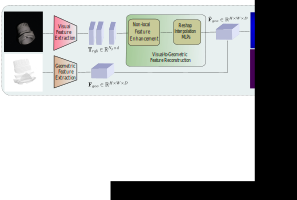
\includegraphics[width=\linewidth]{figs/overview}
\caption{Overview of the proposed unsupervised anomaly detection framework. The method extracts 2D visual features from RGB images and 3D geometric features from point clouds. A Visual-to-Geometric Feature Reconstruction network predicts geometric features from visual inputs, and significant discrepancies indicate anomalies.}
\label{fig:view}
\end{figure*}

Let $\mathbf{I} \in \mathbb{R}^{H \times W \times 3}$ represent an RGB image, where $H$ and $W$ denote the height and width of the image, and the 3 channels correspond to the color information. Let $\mathbf{D} \in \mathbb{R}^{H \times W}$ represent the corresponding depth image, which is pixel-registered with $\mathbf{I}$. This means that each pixel $(u, v)$ in $\mathbf{D}$ corresponds to a pixel in $\mathbf{I}$, providing a depth value $d_{u,v}$ for each valid pixel. From the depth image $\mathbf{D}$, we generate a 3D point cloud $\mathbf{P} = \{(x_i, y_i, z_i)\}_{i=1}^{M}$, where $M$ is the number of valid depth points and each point $(x_i, y_i, z_i)$ represents the 3D coordinates derived from the depth information.

As shown in Figure \ref{fig:view} the objective of the proposed method is to detect anomalies by predicting the 3D geometric features $\hat{\mathbf{F}}_{geo}$ from the 2D visual features $\mathbf{F}_{vis}$ and comparing them with the actual geometric features $\mathbf{F}_{geo}$ extracted from the point cloud. First, the visual features $\mathbf{F}_{vis} \in \mathbb{R}^{H \times W \times d}$ are extracted from the RGB image $\mathbf{I}$ using a Vision Transformer (ViT), capturing the appearance of the object in 2D space. Then, the 3D geometric features $\mathbf{F}_{geo} \in \mathbb{R}^{H \times W \times d}$ are obtained from the depth image $\mathbf{D}$ using a pre-trained 3D model. The core of the method is the geometric feature reconstruction network, which predicts the geometric features $\hat{\mathbf{F}}_{geo}$ from the visual inputs $\mathbf{F}_{vis}$. During training, the network minimizes the difference between the predicted geometric features $\hat{\mathbf{F}}_{geo}$ and the actual geometric features $\mathbf{F}_{geo}$ by minimizing the loss $\mathcal{L}_{geo}$. This process allows the network to learn the normal correlations between 2D visual data and 3D geometric data. During inference, anomalies are detected by comparing the predicted geometric features $\hat{\mathbf{F}}_{geo}$ with the actual geometric features $\mathbf{F}_{geo}$. Significant deviations between these features, measured using the Euclidean distance or another discrepancy measure, indicate abnormal regions in the object.

\subsection*{3D Point Cloud Feature Extraction}

The 3D point cloud $\mathbf{P} = \{(x_i, y_i, z_i)\}_{i=1}^{M}$ is processed using a Masked Autoencoder (MAE) \cite{pang2022masked}. The point cloud is first divided into patches using Farthest Point Sampling (FPS) and K-Nearest Neighbors (KNN). FPS selects $n$ points as patch centers, and KNN selects the $k$ nearest neighbors for each center:

\begin{equation}
    \mathbf{C_T} = \text{FPS}(\mathbf{P}), \quad \mathbf{C_T} \in \mathbb{R}^{n \times 3}\DIFaddbegin \DIFadd{.
}\DIFaddend \end{equation}
\begin{equation}
    \mathbf{P}_{patch} = \text{KNN}(\mathbf{P}, \mathbf{C_T}), \quad \mathbf{P}_{patch} \in \mathbb{R}^{n \times k \times 3}\DIFaddbegin \DIFadd{.
}\DIFaddend \end{equation}

\noindent The masked point patches are processed through PointNet \cite{qi2017pointnet} and the autoencoder to produce geometric features $\mathbf{G}_{geom} \in \mathbb{R}^{M \times D}$. The geometric features $\mathbf{G}_{geom} \in \mathbb{R}^{M \times d}$ are produced for each point in the point cloud. Since the 3D point cloud is derived from the depth image $\mathbf{D}$, we know the pixel coordinates $(u_i, v_i)$ of each 3D point $(x_i, y_i, z_i)$, allowing us to map the geometric features back to their corresponding pixel locations in the 2D image. Using this projection, we place the geometric features into a sparse 2D feature map $\mathbf{G}_{map} \in \mathbb{R}^{H \times W \times d}$, where the pixel $(u_i, v_i)$ contains the feature vector for point $i$.

\begin{equation}
\mathbf{G}_{map}[u_i, v_i, :] = \mathbf{G}_{geom}[i, :]\DIFaddbegin \DIFadd{.
}\DIFaddend \end{equation}

\noindent For pixels without corresponding 3D points, we apply interpolation method as in \cite{wang2023multimodal} to propagate geometric features from neighboring pixels:

\begin{equation}
    \mathbf{F}_{geo} = \text{Interpolate}(\mathbf{G}_{map}) \in \mathbb{R}^{H \times W \times D}\DIFaddbegin \DIFadd{.
}\DIFaddend \end{equation}

\subsection*{Visual Feature Extraction}

The RGB image $\mathbf{I}$ is processed using a Vision Transformer (ViT) \cite{dosovitskiy2020image} to extract high-level visual features. The image $\mathbf{I}$ is divided into non-overlapping patches of size $p \times p$, and each patch is flattened into a vector. A linear projection is applied to embed the patches into a $d$-dimensional feature space:

\begin{equation}
    \mathbf{x}_p = \text{Flatten}(\mathbf{I}) \in \mathbb{R}^{(H \times W) / p^2 \times (p \times p \times 3)}\DIFaddbegin \DIFadd{.
}\DIFaddend \end{equation}

\noindent The set of embedded patches is passed through the transformer encoder to obtain RGB feature tokens:

\begin{equation}
    \mathbf{T}_{rgb} = ViT(\mathbf{x}_p) \in \mathbb{R}^{N_p \times d}\DIFaddbegin \DIFadd{,
}\DIFaddend \end{equation}

\noindent where $N_p = \frac{H \times W}{p^2}$ is the number of patches and $d$ is the dimension of the feature vectors. 

\subsection*{Visual-to-Geometric Feature Reconstruction}

\begin{figure*}[ht]
\centering
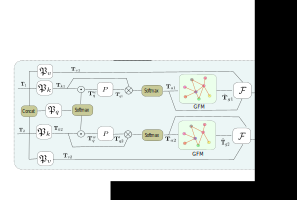
\includegraphics[width=0.8\linewidth]{figs/NL}
\caption{The proposed visual feature enhancement module $\mathcal{M}_{FE}$ used in geometric feature reconstruction. The module \DIFdelbeginFL \DIFdelFL{improves local feature representation through }\DIFdelendFL \DIFaddbeginFL \DIFaddFL{incorporates }\DIFaddendFL non-local attention and graph convolutional networks \DIFaddbeginFL \DIFaddFL{to improve the interaction between global and local features}\DIFaddendFL .}
\label{fig:NL}
\end{figure*}

\DIFdelbegin \DIFdel{While transformers excel at }\DIFdelend \DIFaddbegin \DIFadd{The Visual-to-Geometric Feature Reconstruction network serves as the core of the proposed method, learning to reconstruct 3D geometric features from 2D visual inputs. This approach leverages the complementary nature of appearance and geometric information, enabling precise anomaly detection without the need for direct multimodal fusion. 
}

\DIFadd{Transformers are well-suited for }\DIFaddend capturing global contextual information across \DIFdelbegin \DIFdel{the entire image, they often fall short when it comes to efficiently modeling local interactions . This becomes particularly problematic }\DIFdelend \DIFaddbegin \DIFadd{visual tokens; however, their ability to model localized interactions remains limited. This limitation is particularly critical }\DIFaddend in anomaly detection, where \DIFdelbegin \DIFdel{distinguishing between normal and anomalous regions requires }\DIFdelend fine-grained \DIFdelbegin \DIFdel{analysis due to their often subtle differences. As a result, a combined approach that leverages both global context and local feature interactions is critical for achieving accurate detection}\DIFdelend \DIFaddbegin \DIFadd{deviations often indicate defects}\DIFaddend . To address this\DIFdelbegin \DIFdel{challenge, we introduce }\DIFdelend \DIFaddbegin \DIFadd{, we integrate }\DIFaddend a visual feature enhancement module $\mathcal{M}_{FE}$ \DIFdelbegin \DIFdel{that enhances the geometric feature reconstruction process by improving local feature representation (see Figure\ref{fig:NL}). Inspired by the works of \cite{te2020edge, wang2018non}, this module applies specialized operations to neighboring tokens, ensuring that localized details are preserved alongside the global context . The enhancement process begins with a }\DIFdelend \DIFaddbegin \DIFadd{(Figure~\ref{fig:NL}) within the reconstruction network. This module enhances local feature representations while retaining global context by combining }\DIFaddend non-local \DIFdelbegin \DIFdel{operation, which aggregates information from surrounding tokens to capture broader context and potential anomaly signals. Following this, a graph convolutional network (GCN) is employed to further explore the higher-order semantic relationships between neighboring tokens, allowing the model to detect subtle deviations that may indicate anomalies. The proposed enhancement method is particularly suitable for anomaly detection because anomalies typically manifest as small, localized changes in texture, structure, or geometry. The }\DIFdelend \DIFaddbegin \DIFadd{attention \cite{wang2018non} with graph convolutional networks (GCNs) \cite{defferrard2016convolutional, te2020edge}. The combination of }\DIFaddend non-local \DIFdelbegin \DIFdel{operation ensures that the model can effectively consider both distant and nearby features , enabling it to detect anomalies that are not easily distinguishable based on local patterns alone.
Meanwhile, the GCN enhances the model's ability to focus on higher-level semantic differences by refining local interactions, making it more sensitive to the fine-grained irregularities that characterize anomalies. Together, these operations create a robust system capable of detecting even subtle anomalies in complex industrial settings. }\DIFdelend \DIFaddbegin \DIFadd{attention and graph convolutional networks (GCNs) was chosen to effectively address the complementary aspects of global and local feature integration. Non-local attention captures long-range dependencies across the entire image, which is critical for identifying correlations in visual features across spatially distant regions. GCNs, on the other hand, excel at modeling local relationships and refining features based on neighborhood structures.
}\DIFaddend 

\DIFaddbegin \paragraph*{\DIFadd{Non-Local Attention for Global Context}}
\DIFadd{Non-local attention \cite{wang2018non} captures relationships between spatially distant visual tokens, providing the network with a global understanding of correlations in visual features. }\DIFaddend Specifically, given two neighboring tokens $\mathbf{T}_1$ and $\mathbf{T}_2$ \DIFdelbegin \DIFdel{from visual feature extraction, they are normalized. For instance, }\DIFdelend \DIFaddbegin \DIFadd{extracted from a Vision Transformer, the attention mechanism refines }\DIFaddend $\mathbf{T}_1$ \DIFdelbegin \DIFdel{is passed through two linear projection functions, $\mathfrak{P}_v$ and $\mathfrak{P}_k$, yielding dimension-reduced sequences $\mathbf{T}_v$ and $\mathbf{T}_k$ ($\mathbf{T}_v \in \mathbb{R}^{N_p \times \frac{d}{2}}$ and $\mathbf{T}_k \in \mathbb{R}^{N_p \times \frac{d}{2}}$)}\DIFdelend \DIFaddbegin \DIFadd{as follows}\DIFaddend :

\DIFdelbegin \[
\DIFdel{\mathbf{T}_v = \mathfrak{P}_v(\mathbf{T}_1), \quad \mathbf{T}_k = \mathfrak{P}_k(\mathbf{T}_1)
}\]
%DIFAUXCMD
\DIFdelend \DIFaddbegin \begin{equation}
\DIFadd{\mathbf{T}_v = \mathfrak{P}_v(\mathbf{T}_1), \quad \mathbf{T}_k = \mathfrak{P}_k(\mathbf{T}_1),
}\end{equation}
\DIFaddend 

\noindent \DIFdelbegin \DIFdel{Next, }\DIFdelend \DIFaddbegin \DIFadd{where $\mathfrak{P}_v$ and $\mathfrak{P}_k$ are linear projection layers reducing the dimensionality of $\mathbf{T}_1$ to $\frac{d}{2}$. }\DIFaddend $\mathbf{T}_1$ and $\mathbf{T}_2$ are concatenated to form \DIFdelbegin \DIFdel{an integrated token }\DIFdelend $\mathbf{T}_q$\DIFdelbegin \DIFdel{. A linear projection }\DIFdelend \DIFaddbegin \DIFadd{, and the attention weights are computed as:
}

\begin{equation}
\DIFadd{\mathbf{T}_q^w = \text{softmax}(\mathfrak{P}_q(\mathbf{T}_q)), \quad \mathbf{T}_q' = P\left(\mathbf{T}_k \odot \mathbf{T}_q^w\right),
}\end{equation}

\noindent \DIFadd{where }\DIFaddend $\mathfrak{P}_q$ \DIFdelbegin \DIFdel{reduces its dimension to $\frac{d}{2}$, and a softmax function produces a weight map $\mathbf{T}_q^w$. This map is element-wise multiplied with $\mathbf{T}_k$, followed by }\DIFdelend \DIFaddbegin \DIFadd{projects $\mathbf{T}_q$ to a lower dimension, and $P(\cdot)$ is }\DIFaddend adaptive average pooling\DIFdelbegin \DIFdel{$P(\cdot)$ to reduce computational cost:
}%DIFDELCMD < 

%DIFDELCMD < %%%
\[
\DIFdel{\mathbf{T}_q' = F_1(\mathbf{T}_k, \mathbf{T}_q) = P\left(\mathbf{T}_k \odot \text{softmax}(\mathfrak{P}_q(\mathbf{T}_q))\right)
}\]
%DIFAUXCMD
%DIFDELCMD < 

%DIFDELCMD < \noindent %%%
\DIFdel{A matrix product between $\mathbf{T}_k$ and $\mathbf{T}_q'$ explores their correlation, followed by a softmax operation to generate an }\DIFdelend \DIFaddbegin \DIFadd{. The }\DIFaddend attention map $\mathbf{T}_a$ \DIFaddbegin \DIFadd{is derived from the interaction}\DIFaddend :

\DIFdelbegin \[
\DIFdel{\mathbf{T}_a = \text{softmax}\left(\mathbf{T}_q' \otimes \mathbf{T}_k^\top\right)
}\]
%DIFAUXCMD
%DIFDELCMD < 

%DIFDELCMD < \noindent %%%
\DIFdel{Following \cite{te2020edge}, the attention map $\mathbf{T}_a$ and token $\mathbf{T}_v$ are passed to a graph fusion module (GFM) . In GFM, $\mathbf{T}_v$ is projected onto the graph domain using $\mathbf{T}_a$:
}%DIFDELCMD < 

%DIFDELCMD < %%%
\[
\DIFdel{\mathbf{T}_g = \mathbf{T}_v \otimes \mathbf{T}_a^\top
}\]
%DIFAUXCMD
\DIFdelend \DIFaddbegin \begin{equation}
\DIFadd{\mathbf{T}_a = \text{softmax}(\mathbf{T}_q' \otimes \mathbf{T}_k^\top).
}\end{equation}
\DIFaddend 

\DIFdelbegin %DIFDELCMD < \noindent %%%
\DIFdel{In this step, pixels with similar featuresare grouped into a vertex, and a single-layer GCN learns high-level semantic relations and non-local representations. The vertex features $\mathbf{T}_g$ undergo a spectral graph convolution, producing}\DIFdelend \DIFaddbegin \paragraph*{\DIFadd{Graph Convolutional Networks for Local Interactions}}
\DIFadd{Local interactions between visual features are refined using a graph convolutional network (GCN) \cite{te2020edge}. Tokens are projected into a graph representation where vertices represent similar features, and edges encode relationships. The refined token $\hat{\mathbf{T}}_g$ is computed as}\DIFaddend :

\DIFdelbegin \[
\DIFdel{\hat{\mathbf{T}}_g = \text{ReLU}\left((I - A)\mathbf{T}_g w_g\right)
}\]
%DIFAUXCMD
\DIFdelend \DIFaddbegin \begin{equation}
\DIFadd{\hat{\mathbf{T}}_g = \text{ReLU}\left((I - A)\mathbf{T}_g w_g\right),
}\end{equation}
\DIFaddend 

\noindent where \DIFaddbegin \DIFadd{$\mathbf{T}_g = \mathbf{T}_v \otimes \mathbf{T}_a^\top$, }\DIFaddend $A$ is the adjacency matrix\DIFdelbegin \DIFdel{representing graph connectivity, and $w_g \in \mathbb{R}^{p \times p}$ }\DIFdelend \DIFaddbegin \DIFadd{, and $w_g$ }\DIFaddend is the GCN weight matrix. \DIFdelbegin \DIFdel{Finally, a skip connection combines the input token $\mathbf{T}_1$ with the enhanced representation}\DIFdelend \DIFaddbegin \DIFadd{A skip connection integrates global and local refinements}\DIFaddend :

\DIFdelbegin \[
\DIFdel{\mathbf{T}_{1}^{e} = \mathcal{F}_2(\hat{\mathbf{T}}_g, \mathbf{T}_a, \mathbf{T}_1) = \hat{\mathbf{T}}_g \otimes \mathbf{T}_a^\top + \mathbf{T}_1
}\]
%DIFAUXCMD
\DIFdelend \DIFaddbegin \begin{equation}
\DIFadd{\mathbf{T}_1^e = \hat{\mathbf{T}}_g + \mathbf{T}_1.
}\end{equation}
\DIFaddend 

\noindent The same process is applied to other tokens. \DIFdelbegin \DIFdel{Since the number of patches $N_p$ is smaller than the spatial dimensions $H \times W$, each token in $\mathbf{T}^{e}$ corresponds to a $p \times p$ patch in the original image. To restore the resolution of the enhanced features, the tokens $\mathbf{F}_{e}$ are reshaped into a patch-based feature map:
}%DIFDELCMD < 

%DIFDELCMD < %%%
\begin{displaymath}
    \DIFdel{\mathbf{F}_{patches} = \text{Reshape}(\mathbf{T}^{e}) \in \mathbb{R}^{\frac{H}{p} \times \frac{W}{p} \times d}
}\end{displaymath}
%DIFAUXCMD
\DIFdelend \DIFaddbegin \DIFadd{The adjacency matrix $A$ is dynamically constructed based on the similarity of visual tokens in the feature space. Specifically, token similarity is measured using a distance metric, and a thresholding mechanism is applied to determine graph connectivity. This approach ensures that $A$ adapts to the characteristics of each input, capturing relevant local relationships. The GCN's ability to model higher-order interactions and propagate contextual information across connected nodes provides a distinct advantage over simpler feature aggregation methods, particularly in capturing subtle anomalies that span localized regions.
}\DIFaddend 

\DIFdelbegin %DIFDELCMD < \noindent %%%
\DIFdel{Next, the patch-based feature map is upsampled using bilinear interpolation }\DIFdelend \DIFaddbegin \paragraph*{\DIFadd{Reconstruction of Geometric Features}}
\DIFadd{The enhanced visual features $\mathbf{T}^e$ are reshaped and upsampled }\DIFaddend to match the \DIFdelbegin \DIFdel{original imageresolution}\DIFdelend \DIFaddbegin \DIFadd{spatial dimensions of the input image}\DIFaddend :

\begin{equation}
\mathbf{F}\DIFdelbegin \DIFdel{_{vis} }\DIFdelend \DIFaddbegin \DIFadd{_{patches} }\DIFaddend = \DIFdelbegin \DIFdel{\text{BilinearUpsample}}\DIFdelend \DIFaddbegin \DIFadd{\text{Reshape}}\DIFaddend (\DIFdelbegin \DIFdel{\mathbf{F}_{patches}}\DIFdelend \DIFaddbegin \DIFadd{\mathbf{T}^e}\DIFaddend ) \in \mathbb{R}\DIFdelbegin \DIFdel{^{H \times W \times d}
}\DIFdelend \DIFaddbegin \DIFadd{^{\frac{H}{p} \times \frac{W}{p} \times d},
}\DIFaddend \end{equation}

\DIFaddbegin \begin{equation}
\DIFadd{\mathbf{F}_{vis} = \text{BilinearUpsample}(\mathbf{F}_{patches}) \in \mathbb{R}^{H \times W \times d}.
}\end{equation}

\DIFaddend \noindent \DIFdelbegin \DIFdel{This ensures spatial alignment of $\mathbf{F}_{vis}$ with the original image dimensions $H \times W$}\DIFdelend \DIFaddbegin \DIFadd{Bilinear upsampling was selected for its simplicity and computational efficiency. While more complex methods, such as learnable upsampling, could potentially improve alignment precision, experiments showed that bilinear upsampling produced negligible artifacts and did not significantly affect the accuracy of the reconstructed geometric features}\DIFaddend . Finally, \DIFaddbegin \DIFadd{$\mathbf{F}_{vis}$ is passed through }\DIFaddend a lightweight MLP \DIFdelbegin \DIFdel{maps the visual feature vector of size $d$ to the geometric feature of size $D$, producing the predicted geometric feature map $\hat{\mathbf{F}}_{geo} \in \mathbb{R}^{H \times W \times D}$. The }\DIFdelend \DIFaddbegin \DIFadd{to predict geometric features $\hat{\mathbf{F}}_{geo}$:
}

\begin{equation}
\DIFadd{\hat{\mathbf{F}}_{geo} = \text{MLP}(\mathbf{F}_{vis}).
}\end{equation}

\paragraph*{\DIFadd{Loss Function}}
\DIFadd{The network minimizes the }\DIFaddend L2 \DIFdelbegin \DIFdel{loss between the predicted and actual geometric features }\DIFdelend \DIFaddbegin \DIFadd{reconstruction loss to align the predicted geometric features $\hat{\mathbf{F}}_{geo}$ with the ground-truth features }\DIFaddend $\mathbf{F}_{geo}$\DIFdelbegin \DIFdel{from the 3D point cloud is minimized during training}\DIFdelend :

\begin{equation}
\mathcal{L}_{geo} = \frac{1}{HWD} \sum_{i=1}^{H} \sum_{j=1}^{W} \sum_{k=1}^{D} \left( \mathbf{F}_{geo}(i, j, k) - \hat{\mathbf{F}}_{geo}(i, j, k) \right)^2\DIFaddbegin \DIFadd{.
}\DIFaddend \end{equation}

\noindent \DIFdelbegin \DIFdel{The network progressively refines the visual features using convolutional layers, residual blocks, and attention mechanisms. By minimizing $\mathcal{L}_{geo}$, the network learns correlations between 2D appearance and 3D structure, making it highly effective for detecting anomalies in }\DIFdelend \DIFaddbegin \DIFadd{By leveraging non-local attention and GCNs, $\mathcal{M}_{FE}$ ensures effective integration of global and local information. This design allows the network to capture subtle deviations in both texture and geometry, resulting in accurate anomaly detection for complex }\DIFaddend industrial settings.
\DIFdelbegin \DIFdel{The combination of attention mechanisms and residual connections ensures the preservation and effective utilization of spatial and channel information during geometric feature prediction.
}\DIFdelend 

\subsection*{Anomaly Localization}

During inference, we use the trained prediction network to predict geometric features from the visual features of test samples. For each sample, we extract the 2D visual features $\mathbf{F}_{vis}$ from the RGB image using the pre-trained 2D model and the 3D geometric features $\mathbf{F}_{geo}$ from the point cloud using the pre-trained 3D model. The visual features $\mathbf{F}_{vis}$ are then passed through the geometric feature prediction network to predict the corresponding geometric features $\hat{\mathbf{F}}_{geo}$. We compute an anomaly map by measuring the difference between the predicted geometric features $\hat{\mathbf{F}}_{geo}$ and the actual geometric features $\mathbf{F}_{geo}$ at each spatial location using the L2 norm:

\begin{equation}
\mathbf{A}_{\text{anomaly}}(i, j) = \|\mathbf{F}_{geo}(i, j) - \hat{\mathbf{F}}_{geo}(i, j)\|_2\DIFaddbegin \DIFadd{.
}\DIFaddend \end{equation}

\noindent This anomaly map $\mathbf{A}_{\text{anomaly}} \in \mathbb{R}^{H \times W}$ indicates the likelihood of anomalies at each spatial location. Regions with higher values represent areas where the predicted geometric features deviate significantly from the actual geometric features, suggesting the presence of anomalies. \DIFaddbegin \DIFadd{The predicted anomaly map is finally smoothed using a Gaussian kernel with $\sigma$=4, following \cite{roth2022towards}. }\DIFaddend To obtain a global anomaly score for each sample, we calculate the maximum value in the \DIFaddbegin \DIFadd{smoothed }\DIFaddend anomaly map:

\begin{equation}
S_{\text{global}} = \max_{i,j} \mathbf{A}_{\text{anomaly}}(i, j)\DIFaddbegin \DIFadd{.
}\DIFaddend \end{equation}

\noindent If the global anomaly score $S_{global}$ exceeds a predefined threshold, the sample is classified as anomalous\DIFaddbegin \DIFadd{. The threshold can be determined as in \cite{bergmann2022mvtec, wang2023multimodal}}\DIFaddend . Additionally, the anomaly map provides spatial localization of anomalies by highlighting regions where the largest deviations occur, enabling a detailed inspection of the anomalous areas. 

%
\section*{Evaluation}
\label{sec:evaluation}

\begin{figure*}[ht]
\centering
\DIFdelbeginFL %DIFDELCMD < \includegraphics[width=\linewidth]{figs/result_rgb}
%DIFDELCMD < \includegraphics[width=\linewidth]{figs/result_pc}
%DIFDELCMD < \includegraphics[width=\linewidth]{figs/result_gt}
%DIFDELCMD < \includegraphics[width=\linewidth]{figs/result_baseline}
%DIFDELCMD < \includegraphics[width=\linewidth]{figs/result_ours}
%DIFDELCMD < %%%
\DIFdelendFL \DIFaddbeginFL \includegraphics[width=0.9\linewidth]{figs/result_rgb}
\includegraphics[width=0.9\linewidth]{figs/result_pc}
\includegraphics[width=0.9\linewidth]{figs/result_gt}
\includegraphics[width=0.9\linewidth]{figs/result_baseline}
\includegraphics[width=0.9\linewidth]{figs/result_ours}
\vspace{-0.2cm}

\begin{flushleft}
 \DIFaddFL{\hspace{1.5cm} Crack \hspace{2.6cm} Cut  \hspace{2.6cm} Crack  \hspace{2.5cm} Cut  \hspace{2.3cm} Cut
 }\end{flushleft}

 \vspace{-0.1cm}
\DIFaddendFL \caption{Qualitative results of anomaly detection \DIFaddbeginFL \DIFaddFL{on MVTec 3D-AD dataset \cite{bergmann2022mvtec}}\DIFaddendFL . From top to bottom: input RGB images, point clouds, ground-truth anomaly segmentations, and anomaly maps obtained by our proposed method without and with the visual feature enhancement module $\mathcal{M}_{FE}$. With $\mathcal{M}_{FE}$, the anomaly is accurately located in row 5.}
\DIFdelbeginFL %DIFDELCMD < \label{fig:results}
%DIFDELCMD < %%%
\DIFdelendFL \DIFaddbeginFL \label{fig:results1}
\end{figure*}
%DIF > -----------------------------------------------

\begin{figure*}[ht]
\centering
\includegraphics[width=0.17\linewidth]{figs/result/carot_rgb}
\includegraphics[width=0.17\linewidth]{figs/result/dowel_rgb}
\includegraphics[width=0.17\linewidth]{figs/result/foam_rgb}
\includegraphics[width=0.17\linewidth]{figs/result/potato_rgb}
\includegraphics[width=0.17\linewidth]{figs/result/tire_rgb}
\vspace{0.2cm}

\includegraphics[width=0.17\linewidth]{figs/result/carot_pc}
\includegraphics[width=0.17\linewidth]{figs/result/dowel_pc}
\includegraphics[width=0.17\linewidth]{figs/result/foam_pc}
\includegraphics[width=0.17\linewidth]{figs/result/potato_pc}
\includegraphics[width=0.17\linewidth]{figs/result/tire_pc}
\vspace{0.2cm}

\includegraphics[width=0.17\linewidth]{figs/result/carot_gt}
\includegraphics[width=0.17\linewidth]{figs/result/dowel_gt}
\includegraphics[width=0.17\linewidth]{figs/result/foam_gt}
\includegraphics[width=0.17\linewidth]{figs/result/potato_gt}
\includegraphics[width=0.17\linewidth]{figs/result/tire_gt}
\vspace{0.2cm}

\includegraphics[width=0.17\linewidth]{figs/result/carot_bl}
\includegraphics[width=0.17\linewidth]{figs/result/dowel_bl}
\includegraphics[width=0.17\linewidth]{figs/result/foam_bl}
\includegraphics[width=0.17\linewidth]{figs/result/potato_bl}
\includegraphics[width=0.17\linewidth]{figs/result/tire_bl}
\vspace{0.2cm}

\includegraphics[width=0.17\linewidth]{figs/result/carot_ours}
\includegraphics[width=0.17\linewidth]{figs/result/dowel_ours}
\includegraphics[width=0.17\linewidth]{figs/result/foam_ours}
\includegraphics[width=0.17\linewidth]{figs/result/potato_ours}
\includegraphics[width=0.17\linewidth]{figs/result/tire_ours}
\vspace{-0.1cm}
\begin{flushleft}
 \DIFaddFL{\hspace{1.8cm} Hole \hspace{2.6cm} Bent  \hspace{2.3cm} Cut  \hspace{2.0cm} Hole and Cut  \hspace{1.0cm} Contamination
 }\end{flushleft} 

\vspace{-0.1cm}
\caption{\DIFaddFL{Additional qualitative results of anomaly detection on MVTec 3D-AD dataset \cite{bergmann2022mvtec}. From top to bottom: input RGB images, point clouds, ground-truth anomaly segmentations, and anomaly maps obtained by our proposed method without and with the visual feature enhancement module $\mathcal{M}_{FE}$. With $\mathcal{M}_{FE}$, the anomaly is accurately located in row 5.}}
\label{fig:results2}
\DIFaddendFL \end{figure*}
%DIF > ---------------------------------------------
\DIFaddbegin 

\begin{figure}[ht]
\centering
\includegraphics[width=0.28\linewidth]{figs/eyecandies/29_image_5}
\includegraphics[width=0.28\linewidth]{figs/eyecandies/41_image_4}
\includegraphics[width=0.28\linewidth]{figs/eyecandies/45_image_5}
\vspace{0.2cm}

\includegraphics[width=0.28\linewidth]{figs/eyecandies/29_depth}
\includegraphics[width=0.28\linewidth]{figs/eyecandies/41_depth}
\includegraphics[width=0.28\linewidth]{figs/eyecandies/45_depth}
\vspace{0.2cm}

\includegraphics[width=0.28\linewidth]{figs/eyecandies/29_normals}
\includegraphics[width=0.28\linewidth]{figs/eyecandies/41_normals}
\includegraphics[width=0.28\linewidth]{figs/eyecandies/45_normals}
\vspace{0.2cm}

\includegraphics[width=0.28\linewidth]{figs/eyecandies/29_mask}
\includegraphics[width=0.28\linewidth]{figs/eyecandies/41_mask}
\includegraphics[width=0.28\linewidth]{figs/eyecandies/45_mask}
\vspace{0.2cm}

\includegraphics[width=0.28\linewidth]{figs/eyecandies/29_ours}
\includegraphics[width=0.28\linewidth]{figs/eyecandies/41_ours}
\includegraphics[width=0.28\linewidth]{figs/eyecandies/45_ours}

\caption{\DIFaddFL{Additional qualitative results of anomaly detection on synthetic data. From top to bottom: input RGB images, the rendered depth and normal maps, ground-truth anomaly segmentations, and anomaly maps obtained by our proposed method without and with the visual feature enhancement module $\mathcal{M}_{FE}$. With $\mathcal{M}_{FE}$, the anomaly is accurately located in row 5.}}
\label{fig:results3}
\end{figure}
%DIF > ---------------------------------------------
\DIFaddend 

\subsection*{Experimental Details}

\textbf{Dataset.}  Most existing industrial anomaly detection datasets \DIFdelbegin \DIFdel{provides }\DIFdelend \DIFaddbegin \DIFadd{provide only }\DIFaddend 2D RGB images without corresponding 3D point cloud data. In contrast, 3D industrial anomaly detection is still in its early stages. The MVTec 3D-AD dataset \cite{bergmann2022mvtec} is the first \DIFdelbegin \DIFdel{3D dataset }\DIFdelend \DIFaddbegin \DIFadd{dataset designed specifically }\DIFaddend for industrial anomaly detection \DIFdelbegin \DIFdel{. Following previous works \cite{wang2023multimodal}, we conduct our experiments on this dataset, which is designed to reflect }\DIFdelend \DIFaddbegin \DIFadd{using 3D data. It consists of 4147 scans acquired by a high-resolution industrial 3D sensor (Zivid One+ Medium) under conditions similar to }\DIFaddend real-world \DIFdelbegin \DIFdel{industrial inspection scenarios}\DIFdelend \DIFaddbegin \DIFadd{inspection setups}\DIFaddend . The dataset includes 10 categories of industrial objects, comprising 2656 training samples, 294 validation samples, and 1197 test samples. The \DIFdelbegin \DIFdel{3D scanswere captured using a structured light-based industrial sensor, where the position information is stored in three-channel tensors representing x, y, and z coordinates. Each sample includes both RGB images and pixel-registered 3D information, providing a rich datasetfor experiments.  
The object categories vary from items with natural variations (e.
    g.
    , bagels, carrots, peaches) to more rigid and structured items (e.g.
}\DIFdelend \DIFaddbegin \DIFadd{training and validation sets contain only anomaly-free scans}\DIFaddend , \DIFdelbegin \DIFdel{cable glands, dowels). The test set contains simulated }\DIFdelend \DIFaddbegin \DIFadd{while the test set includes both anomaly-free and anomalous samples.  
}

\DIFadd{The anomalies in the dataset include a wide range of }\DIFaddend real-world \DIFdelbegin \DIFdel{defects such as scratches, dents, holes, contaminations, and deformations, with ground-truth annotations provided for each anomalous sample}\DIFdelend \DIFaddbegin \DIFadd{defect types, such as scratches, dents, contaminations, cracks, holes, and deformations. These defects were devised and fabricated to closely simulate actual defects encountered in industrial settings. For example, the bagel and cookie categories feature cracks, while the carrot exhibits a hole, and the peach and rope contain contaminations. Prototypical examples of anomalies from the dataset's 41 distinct defect types are shown in \cite{bergmann2022mvtec}.  
}

\DIFadd{The dataset's 10 object categories can be grouped based on their properties:
}\begin{itemize}
    \item \DIFadd{\textit{Natural Variations:} Bagel, carrot, cookie, peach, and potato exhibit significant natural variations in shape, size, and texture.
    }\item \DIFadd{\textit{Deformable Objects:} Foam, rope, and tire have standardized appearances but can easily deform.
    }\item \DIFadd{\textit{Rigid Objects:} Cable gland and dowel are rigid and could, in principle, be inspected using CAD models, but the dataset is designed to test unsupervised methods that can handle all object types.
}\end{itemize}

\DIFadd{Each scan includes a pixel-aligned RGB image and a point cloud containing x, y, and z coordinates, which enables a one-to-one mapping between the 2D image and the 3D geometric data. The scans were cropped to a fixed rectangular domain to minimize background pixels while retaining sufficient margins for data augmentation techniques such as cropping, translation, and rotation. The preprocessing ensures consistency with real-world scenarios, where objects are typically positioned in predefined locations with controlled lighting. The acquisition setup features an indirect and diffuse light source, with the sensor statically mounted to maintain a consistent view for each object category. Calibration of internal camera parameters ensures precise projection of 3D points into their corresponding 2D pixel coordinates. This configuration not only aligns with real-world practices but also simplifies data augmentation and preprocessing}\DIFaddend . \\

\noindent \textbf{Implementation Details\footnote{Our code and other materials are available at \url{https://github.com/hoangcuongbk80/GeoAD}}.} Following \cite{wang2023multimodal}, we apply the RANSAC algorithm \cite{fischler1981random} to estimate the background plane, discarding any points within a distance of 0.005 units. For feature extraction, we utilize frozen Transformers as in \cite{wang2023multimodal}. Specifically, we employ DINO ViT-B/8 \cite{dosovitskiy2020image} pre-trained on ImageNet \cite{deng2009imagenet} for visual feature extraction, and Point-MAE \cite{pang2022masked} pre-trained on ShapeNet \cite{chang2015shapenet} for geometric feature extraction. 
\DIFaddbegin 

\DIFaddend The visual feature extraction module processes RGB images of resolution $224 \times 224$, \DIFdelbegin \DIFdel{producing }\DIFdelend \DIFaddbegin \DIFadd{dividing them into non-overlapping patches of size $8 \times 8$. Each patch is flattened and passed through a linear embedding layer, resulting in a $768$-dimensional feature vector per patch. The embedded patches are fed into a Vision Transformer encoder comprising 12 layers of self-attention and feedforward blocks. This produces }\DIFaddend a $28 \times 28 \times 768$ feature map, which is \DIFdelbegin \DIFdel{then upsampled to $224 \times 224 \times 768$ }\DIFdelend \DIFaddbegin \DIFadd{subsequently upsampled }\DIFaddend using bilinear interpolation \DIFdelbegin \DIFdel{before being passed to the geometric feature reconstruction module.
}\DIFdelend \DIFaddbegin \DIFadd{to $224 \times 224 \times 768$ for spatial alignment with the geometric features. Bilinear interpolation uses a scale factor dynamically computed based on the input and output resolutions.
}

\DIFaddend For the point cloud data, we sample 1024 groups of 32 points using Farthest Point Sampling (FPS) \cite{qi2017pointnet++}, \DIFdelbegin \DIFdel{yielding }\DIFdelend \DIFaddbegin \DIFadd{followed by K-Nearest Neighbors (KNN) to define local neighborhoods for each sampled point. Each group is processed through a Masked Autoencoder (Point-MAE) \cite{pang2022masked} to generate }\DIFaddend a $1152$-dimensional \DIFdelbegin \DIFdel{feature vector for each group. These feature vectors }\DIFdelend \DIFaddbegin \DIFadd{geometric feature vector. These features }\DIFaddend are interpolated and aligned to a $224 \times 224 \times 1152$ grid \DIFdelbegin \DIFdel{, which serves as the target }\DIFdelend \DIFaddbegin \DIFadd{using the pixel correspondence between the depth image and the RGB image.
}

\DIFadd{The Visual-to-Geometric Feature Reconstruction module is designed to map the visual features ($224 \times 224 \times 768$) to the }\DIFaddend geometric feature map \DIFdelbegin \DIFdel{for reconstruction. The geometric feature reconstruction module is composed of }\DIFdelend \DIFaddbegin \DIFadd{($224 \times 224 \times 1152$). This module begins by refining the visual features using the visual feature enhancement module $\mathcal{M}_{FE}$, which combines non-local attention and graph convolutional networks (GCNs) to enhance both global and local feature interactions. Specifically:
}\begin{itemize}
    \item \DIFadd{\textbf{Non-Local Attention:} Visual tokens are passed through linear projection layers to compute query, key, and value matrices with dimensions of $384$ each, i.e., $d/2$ where $d = 768$. Attention weights are computed as described in Equation (4) of the paper, and the refined tokens are aggregated using adaptive average pooling with a kernel size of $2 \times 2$. This ensures efficient computation while preserving salient features.
    }\item \DIFadd{\textbf{Graph Convolutional Networks (GCNs):} The adjacency matrix for the GCN is constructed dynamically based on cosine similarity between tokens, with a threshold of 0.6 to retain meaningful connections. A single-layer graph convolution propagates contextual information across connected nodes, using a ReLU activation for non-linearity. The GCN weight matrix $w_g$ has dimensions $8 \times 8$, corresponding to the patch size.
}\end{itemize}

\DIFadd{The refined visual features are reshaped into patch-based feature maps and bilinearly upsampled to match the original spatial resolution ($224 \times 224$). These features are then passed through a lightweight Multi-Layer Perceptron (MLP) comprising }\DIFaddend three fully connected layers with GeLU activation functions\DIFdelbegin \DIFdel{applied after the first two layers. The layers have 768, 960, and 1152 units}\DIFdelend \DIFaddbegin \DIFadd{. The dimensions of the MLP layers are $768$, $960$, and $1152$}\DIFaddend , respectively. \DIFdelbegin \DIFdel{We train the network }\DIFdelend \DIFaddbegin \DIFadd{Dropout with a rate of $0.1$ is applied after each layer to prevent overfitting, and the final output is a predicted geometric feature map $\hat{\mathbf{F}}_{geo}$ aligned with the extracted geometric features $\mathbf{F}_{geo}$.
}

\DIFadd{\textbf{Training Details:} The network is trained }\DIFaddend for 200 epochs using the Adam optimizer \cite{kingma2014adam} with \DIFdelbegin \DIFdel{a }\DIFdelend \DIFaddbegin \DIFadd{an initial }\DIFaddend learning rate of 0.001 \DIFdelbegin \DIFdel{. }\DIFdelend \DIFaddbegin \DIFadd{and a cosine annealing scheduler. The training loss is the L2 reconstruction loss (Equation 6), which minimizes the Euclidean distance between the predicted and actual geometric features. A batch size of 16 is used to balance memory efficiency and convergence speed. Data augmentation techniques, including random cropping and rotation, are applied to enhance generalization.
}

\DIFadd{\textbf{Hardware and Software:} }\DIFaddend All experiments are conducted on a single NVIDIA GeForce RTX 4090 GPU \DIFdelbegin \DIFdel{, utilizing both our implementation and }\DIFdelend \DIFaddbegin \DIFadd{with 24GB of memory. The implementation is based on PyTorch 2.0, and training runs are logged using the Weights and Biases library for performance monitoring. We also validate our results using }\DIFaddend the original authors' code for \DIFaddbegin \DIFadd{a fair }\DIFaddend comparison. \\

\noindent \textbf{Evaluation Metrics.} Following \cite{bergmann2022mvtec, wang2023multimodal}, we employ two metrics: the Image-level Area Under the Receiver Operating Characteristic curve (I-AUROC) and the Area Under the Per-Region Overlap curve (AUPRO). These metrics provide insights into both anomaly classification and localization performance. I-AUROC is used to assess the model's ability to classify an entire test image as either anomaly-free or containing an anomaly. The AUROC curve is derived by plotting the true positive rate (TPR) against the false positive rate (FPR) at various threshold levels. The I-AUROC score provides a threshold-independent evaluation of the model's classification performance, with a score of 1 indicating perfect classification. A higher I-AUROC score signifies better image-level anomaly detection performance. AUPRO evaluates the model's ability to localize anomalies within the test samples. AUPRO measures how well the predicted anomaly regions overlap with the ground truth at different thresholds, thus reflecting the model's localization accuracy. For each connected component \( C_k \) in the ground truth, the overlap between the binary prediction \( P \) and \( C_k \) is computed. The Per-Region Overlap (PRO) for each region is defined as:
\begin{equation}
    \text{PRO}(C_k) = \frac{|P \cap C_k|}{|C_k|}
\end{equation}
AUPRO is computed by integrating the PRO over a range of thresholds, typically up to a false positive rate (FPR) limit.  We report the area under the PRO curve with an upper integration limit of 0.3 as in \cite{bergmann2022mvtec}. By focusing on localization performance, AUPRO offers a more precise evaluation of anomaly detection in complex industrial settings, where accurately pinpointing defect regions is critical. These metrics together provide a comprehensive view of the model's ability to detect and localize anomalies.

\subsection*{Results}

\begin{table*}[ht]
\centering
\begin{tabular}{cl|r|r|r|r|r|r|r|r|r|r|r}
\hline
& Method & Bagel & \makecell{Cable \\ Gland} & Carrot & Cookie & Dowel & Foam & Peach & Potato & Rope & Tire & Mean \\
\hline
\parbox[t]{0.5mm}{\multirow{8}{*}{\rotatebox[origin=c]{90}{3D}}} & Depth GAN & 0.530 & 0.376 & 0.607 & 0.603 & 0.497 & 0.484 & 0.595 & 0.489 & 0.536 & 0.521 & 0.523 \\
& Voxel AE & 0.693 & 0.425 & 0.515 & 0.790 & 0.494 & 0.558 & 0.537 & 0.484 & 0.639 & 0.583 & 0.571 \\
& Depth AE & 0.468 & 0.731 & 0.497 & 0.673 & 0.534 & 0.417 & 0.485 & 0.549 & 0.564 & 0.546 & 0.546 \\
& Voxel VM & 0.750 & 0.747 & 0.613 & 0.738 & 0.823 & 0.693 & 0.679 & 0.652 & 0.609 & 0.690 & 0.699 \\
& Depth VM & 0.510 & 0.542 & 0.469 & 0.576 & 0.609 & 0.699 & 0.450 & 0.419 & 0.668 & 0.520 & 0.546 \\
& FPFH & 0.825 & 0.551 & 0.952 & 0.797 & 0.883 & 0.582 & 0.758 & 0.889 & 0.929 & 0.653 & 0.782 \\
& Voxel GAN & 0.383 & 0.623 & 0.474 & 0.639 & 0.564 & 0.409 & 0.617 & 0.427 & 0.663 & 0.577 & 0.537 \\
& AST & 0.881 & 0.576 & 0.965 & 0.957 & 0.679 & 0.797 & \textbf{0.990} & 0.915 & 0.956 & 0.611 & 0.833 \\
& 3D-ST & 0.862 & 0.484 & 0.832 & 0.894 & 0.848 & 0.663 & 0.763 & 0.687 & 0.958 & 0.486 & 0.748 \\
& M3DM & 0.941 & 0.651 & 0.965 & 0.969 & 0.905 & 0.760 & 0.880 & 0.974 & 0.926 & 0.765 & 0.874 \\
\hline
\parbox[t]{0.5mm}{\multirow{3}{*}{\rotatebox[origin=c]{90}{RGB}}} & DifferNet & 0.859 & 0.703 & 0.643 & 0.435 & 0.797 & 0.790 & 0.787 & 0.643 & 0.715 & 0.590 & 0.696 \\
& STFPM & 0.930 & 0.847 & 0.980 & 0.575 & 0.947 & 0.766 & 0.710 & 0.598 & 0.965 & 0.701 & 0.793 \\
& PADiM & 0.975 & 0.775 & 0.698 & 0.582 & 0.663 & 0.582 & 0.660 & 0.535 & 0.832 & 0.760 & 0.764 \\
& AST & 0.947 & \textbf{0.928} & 0.851 & 0.825 & \underline{0.981} & \underline{0.951} & 0.895 & 0.613 & 0.992 & 0.821 & 0.880 \\
& PatchCore & 0.876 & 0.880 & 0.791 & 0.682 & 0.912 & 0.701 & 0.695 & 0.618  & 0.841 & 0.702 & 0.770 \\
& M3DM & 0.944 & 0.918 & 0.896 & 0.749 & 0.959 & 0.767 & 0.919 & 0.648 & 0.938 & 0.767 & 0.850 \\
\hline
\parbox[t]{0.5mm}{\multirow{8}{*}{\rotatebox[origin=c]{90}{RGB + 3D}}} & Depth GAN & 0.538 & 0.372 & 0.580 & 0.603 & 0.430 & 0.534 & 0.042 & 0.601 & 0.443 & 0.577 & 0.532 \\
& Voxel AE & 0.510 & 0.540 & 0.384 & 0.693 & 0.632 & 0.550 & 0.494 & 0.721 & 0.413 & 0.538 & 0.538 \\
& Depth AE & 0.648 & 0.502 & 0.650 & 0.488 & 0.805 & 0.522 & 0.712 & 0.529 & 0.540 & 0.552 & 0.595 \\
& Voxel VM & 0.553 & 0.772 & 0.484 & 0.701 & 0.751 & 0.578 & 0.480 & 0.466 & 0.689 & 0.611 & 0.609 \\
& Depth VM & 0.513 & 0.551 & 0.477 & 0.581 & 0.617 & 0.716 & 0.450 & 0.421 & 0.598 & 0.623 & 0.555 \\
& AST & 0.983 & 0.873 & 0.976 & 0.971 & 0.932 & 0.885 & 0.974 & 0.981 & \textbf{1.000} & 0.797 & 0.937 \\
& Voxel GAN & 0.680 & 0.324 & 0.565 & 0.509 & 0.599 & 0.579 & 0.601 & 0.482 & 0.601 & 0.482 & 0.517 \\
& 3D-ST & 0.950 & 0.483 & \underline{0.986} & 0.921 & 0.905 & 0.632 & 0.945 & \textbf{0.988} & 0.976 & 0.542 & 0.833 \\
& M3DM & \textbf{0.994} & 0.909 & 0.972 & \underline{0.976} & 0.960 & 0.942 & 0.973 & 0.899 & 0.972 & \underline{0.850} & \underline{0.945} \\
& Ours & \underline{0.990} & \underline{0.922} & \textbf{0.988} & \textbf{0.979} & \textbf{0.984} & \textbf{0.973} & \underline{0.988} & \underline{0.985} & \underline{0.994} & \textbf{0.883} & \textbf{0.968} \\
\hline
\end{tabular}
\caption{\label{tab:1} I-AUROC score for anomaly detection of all categories of MVTec-3D AD. Results FPFH \cite{horwitz2022empirical}, PatchCore \cite{roth2022towards}, PADiM \cite{defard2021padim}, 3D-ST \cite{bergmann2023anomaly}, AST \cite{rudolph2023asymmetric}, DifferNet \cite{rudolph2021same}, STFPM \cite{wang2021student}, M3DM \cite{wang2023multimodal} are obtained from \cite{wang2023multimodal}, and the remaining methods from \cite{bergmann2022mvtec}. Best results in \textbf{bold}, runner-ups \underline{underlined}.}
\end{table*}
%/--------------------------------------------------------------------

Figure \DIFdelbegin \DIFdel{\ref{fig:results} demonstrates }\DIFdelend \DIFaddbegin \DIFadd{\ref{fig:results1} and \ref{fig:results2} demonstrate }\DIFaddend the qualitative performance of our method on the MVTec 3D-AD dataset. In comparison to the baseline, our anomaly maps exhibit significantly sharper localization, aligning closely with the ground-truth defect regions. Table \ref{tab:1} presents the I-AUROC scores for various anomaly detection methods evaluated on the MVTec-3D AD dataset. The proposed method demonstrates good performance across most categories, achieving the highest mean I-AUROC score of 0.968. This performance highlights the model's superior ability to differentiate between normal and anomalous samples. The key reason behind this success lies in the visual-to-geometric feature reconstruction approach, which allows the model to predict geometric features from visual features, thereby learning complex correlations between appearance and structure in normal objects. In comparison to other methods, such as AST \cite{rudolph2023asymmetric} and M3DM \cite{wang2023multimodal}, the proposed model consistently outperforms in many object categories, including Cookie, Dowel, Foam, and Tire, achieving scores of 0.979, 0.984, 0.973, and 0.883, respectively. These high scores demonstrate the efficacy of the Visual-to-Geometric Feature Reconstruction network, which effectively learns the correlation between 2D visual features and 3D geometric features, allowing the model to be highly responsive to irregularities in both the appearance and structure of objects. However, the proposed method does not always perform better than certain RGB-only methods. For instance, in the Cable Gland category, the proposed method achieves an I-AUROC score of 0.922, whereas the RGB-based AST model attains a slightly higher score of 0.928. This discrepancy might be attributed to the nature of the cable gland object, which is characterized by complex geometry and reflective surfaces that can be difficult to accurately measure in 3D. The presence of intricate details and curved surfaces introduces noise and inaccuracies in the 3D point cloud data, leading to suboptimal feature reconstruction and anomaly detection. The RGB-only models, such as AST, is benefit in this case from focusing solely on visual information without the added complexity of geometric features, which might not be reliably captured.

%/--------------------------------------------------------------------
\begin{table*}[ht]
\centering
\begin{tabular}{cl|r|r|r|r|r|r|r|r|r|r|r}
\hline
& Method & Bagel & \makecell{Cable \\ Gland} & Carrot & Cookie & Dowel & Foam & Peach & Potato & Rope & Tire & Mean \\
\hline
\parbox[t]{0.5mm}{\multirow{8}{*}{\rotatebox[origin=c]{90}{3D}}} & Depth GAN & 0.111 & 0.072 & 0.212 & 0.174 & 0.160 & 0.128 & 0.003 & 0.042 & 0.446 & 0.075 & 0.143 \\
& Voxel AE & 0.260 & 0.341 & 0.581 & 0.351 & 0.502 & 0.234 & 0.351 & 0.658 & 0.015 & 0.185 & 0.348 \\
& Depth AE & 0.147 & 0.069 & 0.293 & 0.217 & 0.207 & 0.181 & 0.164 & 0.066 & 0.545 & 0.142 & 0.203 \\
& Voxel VM & 0.453 & 0.343 & 0.521 & 0.697 & 0.680 & 0.284 & 0.349 & 0.634 & 0.616 & 0.346 & 0.492 \\
& FPFH & 0.973 & 0.879 & 0.982 & 0.906 & 0.892 & 0.735 & \underline{0.977} & 0.982 & 0.956 & 0.961 & 0.924 \\
& Depth VM & 0.280 & 0.374 & 0.243 & 0.526 & 0.485 & 0.314 & 0.199 & 0.388 & 0.543 & 0.385 & 0.374 \\
& Voxel GAN & 0.440 & 0.453 & 0.875 & 0.755 & 0.782 & 0.378 & 0.392 & 0.639 & 0.775 & 0.389 & 0.583 \\
& M3DM & 0.943 & 0.818 & 0.977 & 0.882 & 0.881 & 0.743 & 0.958 & 0.974 & 0.950 & 0.929 & 0.906 \\
\hline
\parbox[t]{0.5mm}{\multirow{4}{*}{\rotatebox[origin=c]{90}{RGB}}} & CFlow & 0.855 & 0.919 & 0.958 & 0.867 & 0.969 & 0.500 & 0.889 & 0.935 & 0.904 & 0.919 & 0.871 \\
& PADiM & \textbf{0.980} & 0.944 & 0.945 & 0.925 & 0.961 & 0.792 & 0.966 & 0.940 & 0.937 & 0.912 & \textbf{0.930} \\
& PatchCore & 0.901 & 0.949 & 0.928 & 0.877 & 0.892 & 0.563 & 0.904 & 0.932 & 0.908 & 0.906 & 0.876 \\
& M3DM & 0.952 & \underline{0.972} & 0.973 & 0.891 & 0.932 & 0.843 & 0.970 & 0.956 & 0.968 & \underline{0.966} & 0.942 \\
\hline
\parbox[t]{0.5mm}{\multirow{7}{*}{\rotatebox[origin=c]{90}{RGB+3D}}} & Depth GAN & 0.421 & 0.422 & 0.778 & 0.696 & 0.494 & 0.252 & 0.285 & 0.362 & 0.402 & 0.631 & 0.474 \\
& Voxel AE & 0.467 & 0.721 & 0.918 & 0.405 & 0.550 & 0.019 & 0.918 & 0.019 & 0.170 & 0.564 & 0.471 \\
& Depth AE & 0.432 & 0.158 & 0.808 & 0.491 & 0.841 & 0.406 & 0.262 & 0.216 & 0.716 & 0.478 & 0.481 \\
& Voxel VM & 0.510 & 0.300 & 0.507 & 0.611 & 0.366 & 0.611 & 0.366 & 0.611 & 0.366 & 0.611 & 0.471 \\
& Depth VM & 0.388 & 0.321 & 0.194 & 0.570 & 0.408 & 0.282 & 0.244 & 0.349 & 0.268 & 0.331 & 0.335 \\
& Voxel GAN & 0.664 & 0.620 & 0.766 & 0.740 & 0.783 & 0.332 & 0.582 & 0.790 & 0.633 & 0.483 & 0.639 \\
& 3D-ST & 0.950 & 0.483 & \textbf{0.988} & \underline{0.976} & 0.905 & 0.542 & 0.945 & \textbf{0.988} & \textbf{0.976} & 0.542 & 0.833 \\
& M3DM & 0.970 & 0.971 & 0.979 & 0.973 & \underline{0.981} & \underline{0.950} & 0.973 & 0.981 & 0.973 & 0.950 & \underline{0.964} \\
& Ours & \underline{0.978} & \textbf{0.976} & \underline{0.985} & \textbf{0.983} & \textbf{0.986} & \textbf{0.965} & \textbf{0.981} & \underline{0.985} & \underline{0.975} & \textbf{0.970} & \textbf{0.978} \\
\hline
\end{tabular}
\caption{\label{tab:2} AUPRO score for anomaly localization of all categories of MVTec-3D. Results of FPFH \cite{horwitz2022empirical}, CFlow \cite{gudovskiy2022cflow}, PatchCore \cite{roth2022towards}, PADiM \cite{defard2021padim}, 3D-ST \cite{bergmann2023anomaly}, M3DM \cite{wang2023multimodal} are obtained from \cite{wang2023multimodal}, and the remaining methods from \cite{bergmann2022mvtec}. Best results in \textbf{bold}, runner-ups \underline{underlined}.}
\end{table*}
%/--------------------------------------------------------------------

Table \ref{tab:2} provides the AUPRO scores for anomaly localization across the different categories of the MVTec-3D dataset. The proposed method achieves a high average score of 0.978, indicating its strong ability to localize anomalies accurately. The visual-to-geometric feature reconstruction approach plays a crucial role here by enabling the model to identify the regions where visual and predicted geometric features significantly deviate. The model excels in categories such as Carrot, Cookie, and Dowel, where the AUPRO scores are 0.985, 0.983, and 0.986, respectively. The visual-to-geometric feature reconstruction allows the model to infer the geometric properties that should correspond to specific visual features. This enables it to detect regions where the predicted geometric features deviate from the actual ones, which is particularly effective for accurately localizing anomalies in these categories. By using non-local attention mechanisms, the model can capture global dependencies, while GCNs allow for the refinement of local relationships, ensuring that both large-scale and fine-grained anomalies are effectively localized. However, there are some categories, such as Bagel where RGB-based methods outperform the proposed model. For instance, the RGB-based PADiM achieves a higher AUPRO score of 0.980, respectively, compared to the proposed method's scores of 0.978. The slightly lower performance in these categories is due to the complex textures present in bagels, which can introduce inconsistencies in the depth information. Since the proposed model relies on accurately reconstructing geometric features from visual data, errors in depth estimation can reduce its ability to accurately localize anomalies. 

Overall, the proposed method demonstrates strong performance in anomaly detection and localization by leveraging the visual-to-geometric feature reconstruction approach. This strategy enables the model to learn the correlations between visual and geometric features without directly fusing them, leading to a deep understanding of how visual features relate to their geometric counterparts. The occasional underperformance in certain categories highlights the importance of high-quality geometric data acquisition and accurate depth estimation, which are critical for improving the efficacy of the reconstruction process in complex and reflective objects.

\subsection*{Additional Experiments and Ablation Study}

\DIFaddbegin
%----------------------------------------------------------
\begin{table*}[h]
\centering
\begin{tabular}{l|ccc|ccc|cc}
\hline
& \multicolumn{3}{c|}{Simulation} & \multicolumn{3}{c|}{MVTec 3D-AD}  & Frame Rate  & Memory \\
\hline
& I-AUROC & \text{AUPRO(0.3)} & \text{AUPRO(0.05)} & I-AUROC & \text{AUPRO(0.3)} & \text{AUPRO(0.05)} & FPS & MB \\
\hline
3D-ST \cite{bergmann2023anomaly} & \DIFadd{0.852} & \DIFadd{0.841} & \DIFadd{0.504} & 0.833  & 0.833 & 0.465 & 5.130 & 2504 \\
\hline
M3DM \cite{wang2023multimodal} & \DIFadd{0.948} & \DIFadd{0.974} & \DIFadd{0.542} & 0.945 & 0.964 & 0.521 & 0.514 & 6526 \\
\hline
Ours (-$\mathcal{M}_{FE}$)  & \DIFadd{0.870} & \DIFadd{0.893} & \DIFadd{0.527} & 0.873  & 0.884 & 0.502 & 9.814 & 942 \\
\hline
Ours (-GCN) & \DIFadd{0.925} & \DIFadd{0.936} & \DIFadd{0.599} & 0.914  & 0.920 & 0.551 & 8.801 & 1002 \\
\hline
Ours (-NLA) & \DIFadd{0.913} & \DIFadd{0.932} & \DIFadd{0.568} & 0.905  & 0.912 & 0.542 & 8.762 & 985 \\
\hline
Ours (Full) & \DIFadd{\textbf{0.972}} & \DIFadd{\textbf{0.971}} & \DIFadd{\textbf{0.752}} & \textbf{0.968}  & \textbf{0.978} & \textbf{0.702} & \textbf{8.213} & \textbf{1045} \\
\hline
\end{tabular}
\caption{\label{tab:extra_results} Comparison of anomaly detection performance, inference speed, and memory usage on Simulation and the MVTec 3D-AD dataset. AUPRO(0.3) and AUPRO(0.05) represent area under the per-region overlap curve with False Positive Rate (FPR) thresholds of 0.3 and 0.05, respectively. Frame rate is measured in frames per second (FPS), and memory usage refers to the memory footprint during inference. Ours (-$\mathcal{M}_{FE}$) refers to our method without the visual feature enhancement module.}
\end{table*}
%----------------------------------------------------------
\DIFaddend

\DIFaddbegin \DIFadd{\textbf{Metrics}. }\DIFaddend In Tables \ref{tab:1} and \ref{tab:2}, we use a False Positive Rate (FPR) integration threshold of 0.3 to calculate the AUPRO, which serves as an indicator of anomaly localization performance. However, for real-world industrial applications, a 0.3 FPR threshold may be too tolerant, potentially leading to an excessive number of false positives. In industrial settings, high precision is critical to avoid unnecessary interventions, so a tighter threshold is often preferred. Therefore, in this section, we present additional experiments using a more stringent FPR threshold of 0.05 provides a more realistic evaluation of our model's performance in industrial anomaly detection tasks. To distinguish between the two evaluation settings, we refer to the AUPRO values calculated with FPR thresholds of 0.3 and 0.05 as AUPRO(0.3) and AUPRO(0.05), respectively. 

\DIFdelbegin \DIFdel{Table \ref{tab:extra_results} presents these metrics for various methods on }\DIFdelend \DIFaddbegin \DIFadd{\textbf{Simulation}. We further expanded simulation tests to demonstrate the effectiveness and robustness of the proposed Transformer-based Visual-to-Geometric feature reconstruction module. Following \cite{bonfiglioli2022eyecandies}, we generated a synthetic dataset using the Blender framework, a popular 3D modeling software that provides seamless interoperability with Python via the BlenderProc package. BlenderProc is a procedural synthetic data generation tool that allows for controlled and reproducible creation of 3D environments. Using this framework, we simulated industrial scenarios with various object shapes, textures, lighting conditions, and geometric anomalies. Figure \ref{fig:results3} shows examples of the generated samples. The dataset consists of 10,000 images for training and 1,000 images for testing, with corresponding 3D point cloud data and ground-truth anomaly maps. Models were trained on this dataset using the same hyperparameters as for }\DIFaddend the MVTec 3D-AD dataset, \DIFdelbegin \DIFdel{including comparisons between the full version of our model and its variant without }\DIFdelend \DIFaddbegin \DIFadd{ensuring consistency in training configurations.
}

\DIFadd{\textbf{Configurations}. To evaluate the contributions of different components within the proposed Transformer-based Visual-to-Geometric feature reconstruction module, we implemented the following configurations:
}\begin{itemize}
    \item \DIFadd{\textbf{Ours (-$\mathcal{M}_{FE}$):} The visual features ($224 \times 224 \times 768$) were directly passed to the Multi-Layer Perceptron (MLP) without applying }\DIFaddend the visual feature enhancement module \DIFdelbegin \DIFdel{(}\DIFdelend $\mathcal{M}_{FE}$\DIFdelbegin \DIFdel{).
    Our full method achieves the highest }\DIFdelend \DIFaddbegin \DIFadd{.
    }\item \DIFadd{\textbf{Ours (-GCN):} In this configuration, the graph convolutional network (GCN) is omitted, and only the non-local attention mechanism is used to refine the visual features. Visual tokens are processed through linear projection layers to compute reduced-dimension representations. These are concatenated and passed through adaptive average pooling to compute the attention weights. The attention mechanism aggregates information across spatially distant tokens, producing refined visual features that capture global contextual relationships. These refined features are directly passed to the Multi-Layer Perceptron (MLP) for geometric feature prediction. No steps involving graph adjacency matrix construction or graph convolution are included.
    }\item \DIFadd{\textbf{Ours (-NLA):} In this configuration, the non-local attention mechanism is excluded, and the visual features are refined using the GCN. A graph representation is constructed dynamically by calculating cosine similarity between tokens and applying a threshold to form the adjacency matrix. Tokens are then projected into the graph domain, and graph convolution is applied to propagate information across connected nodes. The output of the GCN is integrated with the original tokens using a skip connection to produce refined visual features. These features are subsequently passed to the MLP for geometric feature prediction, without any attention-based refinement.
    }\item \DIFadd{\textbf{Full Module (Proposed):} Both non-local attention and GCN were used as part of the visual feature enhancement module $\mathcal{M}_{FE}$ to refine the visual features.
}\end{itemize}

\DIFadd{\textbf{Result}. The experimental results are summarized in Table \ref{tab:extra_results}, showcasing the performance of our proposed method and its ablated variants on both the synthetic dataset (Simulation) and the MVTec 3D-AD dataset. Our full method achieved the highest performance across all metrics, with }\DIFaddend I-AUROC \DIFdelbegin \DIFdel{score (0.968) }\DIFdelend \DIFaddbegin \DIFadd{scores of 0.972 }\DIFaddend and \DIFdelbegin \DIFdel{outperforms competing RGB+3D methods such as 3D-ST and M3DM across all metrics. This is particularly evident in the AUPRO(0.05) metric, where we achieve a significant improvement over M3DM (0.702 vs. 0.521).
    This highlights the model's superior anomaly localization capabilities, particularly when a more stringent false positive rate (FPR) threshold is applied. The tighter }\DIFdelend \DIFaddbegin \DIFadd{0.968 on the synthetic and MVTec 3D-AD datasets, respectively. Notably, the }\DIFaddend AUPRO(0.05) \DIFdelbegin \DIFdel{threshold ensures fewer false positives}\DIFdelend \DIFaddbegin \DIFadd{scores of 0.752 on the synthetic dataset and 0.702 on MVTec 3D-AD demonstrate the robustness of our method in scenarios requiring high precision}\DIFaddend , which is critical for \DIFdelbegin \DIFdel{industrial anomaly detection applicationswhere high precision is required. }%DIFDELCMD < 

%DIFDELCMD < %%%
\DIFdelend \DIFaddbegin \DIFadd{real-world industrial applications. }\DIFaddend The ablation study \DIFdelbegin \DIFdel{demonstrates the effectiveness of the proposed }\DIFdelend \DIFaddbegin \DIFadd{reveals that removing the }\DIFaddend visual feature enhancement module \DIFdelbegin \DIFdel{. Without this module, the }\DIFdelend \DIFaddbegin \DIFadd{($\mathcal{M}_{FE}$) resulted in a significant drop in performance, with }\DIFaddend I-AUROC \DIFdelbegin \DIFdel{drops from 0.968 }\DIFdelend \DIFaddbegin \DIFadd{decreasing }\DIFaddend to 0.873 \DIFdelbegin \DIFdel{, and the localization performance also declines}\DIFdelend \DIFaddbegin \DIFadd{and AUPRO(0.05) falling to 0.502 on MVTec 3D-AD. Similarly, excluding the graph convolutional network (GCN) reduced the model's ability to capture fine-grained spatial relationships, leading to an AUPRO(0.05) of 0.551, highlighting the importance of local feature refinement. When the non-local attention mechanism was omitted, performance also declined}\DIFaddend , with AUPRO(\DIFdelbegin \DIFdel{0.3) and }\DIFdelend \DIFaddbegin \DIFadd{0.05) decreasing to 0.542 on MVTec 3D-AD, underscoring the necessity of capturing global dependencies for detecting anomalies spanning large spatial regions.
}

\DIFadd{Compared to baseline methods, our full model outperformed both 3D-ST \cite{bergmann2023anomaly} and M3DM \cite{wang2023multimodal}, achieving a 38.5\% and 13.0\% improvement in }\DIFaddend AUPRO(0.05) \DIFdelbegin \DIFdel{scores decreasing by 0.094 and 0.2}\DIFdelend \DIFaddbegin \DIFadd{on the synthetic dataset}\DIFaddend , respectively. This \DIFdelbegin \DIFdel{significant performance drop underscores the importance of the module in refining local visual features, allowing the model to detect subtle and localized anomalies more effectively. The enhancement module contributes not only to anomaly detection accuracy but also to improved generalization across diverse anomaly types. Despite achieving higher accuracy, our full method maintains a competitive inference speed }\DIFdelend \DIFaddbegin \DIFadd{demonstrates the superiority of our approach in both anomaly localization and overall detection performance. Additionally, our method maintains competitive efficiency, achieving a frame rate }\DIFaddend of 8.213 \DIFdelbegin \DIFdel{FPS-significantly higher than M3DM (0.514 FPS )-while requiring substantially less memory (}\DIFdelend \DIFaddbegin \DIFadd{FPS with a memory footprint of }\DIFaddend 1045 MB\DIFdelbegin \DIFdel{vs. }\DIFdelend \DIFaddbegin \DIFadd{. In contrast, M3DM required significantly more memory (}\DIFaddend 6526 MB\DIFdelbegin \DIFdel{for M3DM) . This indicates that our method is well-suited }\DIFdelend \DIFaddbegin \DIFadd{) while achieving lower frame rates, making our method better suited }\DIFaddend for real-time industrial applications\DIFdelbegin \DIFdel{, offering a balance between high performance and efficiency. The absence of }\DIFdelend \DIFaddbegin \DIFadd{. The results confirm that the integration of non-local attention and GCN in }\DIFaddend the visual feature enhancement module \DIFdelbegin \DIFdel{further increases the frame rate to 9.814 FPS, but at the cost of reduced detection and localization accuracy, as evidenced by the lower I-AUROC and AUPRO scores}\DIFdelend \DIFaddbegin \DIFadd{enables our model to achieve state-of-the-art performance while remaining efficient. The stricter AUPRO(0.05) metric further validates the robustness of our method under high-precision requirements, highlighting its practical applicability in industrial anomaly detection tasks}\DIFaddend .

\section*{Conclusion}
\label{sec:Conclusion}

In this paper, we proposed a novel framework for unsupervised industrial anomaly detection that leverages both 2D visual features and 3D geometric information through a Visual-to-Geometric Feature Reconstruction network. Unlike traditional multimodal approaches that directly fuse features from different modalities, our method predicts 3D geometric features from 2D visual features, enabling the model to learn the correlation between an object's appearance and its geometric structure. This approach allows the model to effectively detect deviations from normalcy, which are indicative of anomalies in both 2D and 3D spaces. Our experimental results demonstrate that the proposed method achieves state-of-the-art performance on the MVTec 3D-AD dataset, outperforming existing methods in both anomaly detection accuracy and localization performance. The model's superior performance, as evidenced by high I-AUROC and AUPRO scores, is particularly notable when applying a more stringent AUPRO(0.05) threshold, which is crucial for real-world industrial applications where precision is paramount. The visual feature enhancement module plays a critical role in our framework, contributing significantly to both detection accuracy and localization precision. Our ablation study shows that removing this module leads to a notable drop in performance, highlighting its importance in refining local feature representation and enabling the model to detect subtle anomalies that might otherwise be missed. Additionally, our method is highly efficient in terms of both inference speed and memory footprint, making it suitable for real-world applications in resource-constrained industrial environments. Despite leveraging both 2D and 3D data, the model maintains competitive frame rates and requires significantly less memory than other multimodal methods, ensuring its practicality in real-world scenarios. Future work could explore extending this approach to more complex anomaly types and further optimizing the model for deployment on edge devices.
%
\bibliographystyle{IEEEtran}
\bibliography{References}

\begin{IEEEbiography}[{\includegraphics[width=1in,height=1.25in,clip,keepaspectratio]{authors/DinhCuong}}]{Dinh-Cuong Hoang} received his Ph.D. degree in computer science from Orebro University, Sweden (2021), and is currently a lecturer at FPT University, Greenwich Vietnam. His research interests lie at the intersection of computer vision, robotics, and machine learning. He is particularly interested in topics involving autonomy for robots, with a focus on perception algorithms.
\end{IEEEbiography}

\begin{IEEEbiography}[{\includegraphics[width=1in,height=1.25in,clip,keepaspectratio]{authors/prof_Tan}}]{Phan Xuan Tan} (Member, IEEE) received the B.E. degree in Electrical-Electronic Engineering from Military Technical Academy, Vietnam, M.E. degree in Computer and Communication Engineering from Hanoi University of Science and Technology, Vietnam and Ph.D. degree in Functional Control Systems from Shibaura Institute of Technology, Japan. He is currently an Associate Professor at Shibaura Institute of Technology. His current research interests include computer vision, deep learning and image processing.
\end{IEEEbiography}

\begin{IEEEbiography}[{\includegraphics[width=1in,height=1.25in,clip,keepaspectratio]{authors/NguyenAnhNhat}}]{Anh-Nhat Nguyen}  is currently a lecturer at FPT University, Vietnam. He received his B.S. and M.S. degrees in Computer Science from Duy Tan University, Da Nang, Vietnam, in 2012 and from Huazhong University of Science and Technology (HUST), China, in 2018, respectively. His research interests include image processing, information security, physical layer secrecy, radio-frequency energy harvesting, and wireless sensor networks.
\end{IEEEbiography}

\begin{IEEEbiography}[{\includegraphics[width=1in,height=1.25in,clip,keepaspectratio]{authors/TranDucThanh}}]{Duc-Thanh Tran} is pursuing a B.S. degree in Artificial Intelligence at FPT University, Hanoi, Vietnam, with a primary focus on research in the field of computer vision.
\end{IEEEbiography}

\begin{IEEEbiography}[{\includegraphics[width=1in,height=1.25in,clip,keepaspectratio]{authors/DuongVanHiep}}]{Van-Hiep Duong} is pursuing a B.S. degree in Artificial Intelligence at FPT University, Hanoi, Vietnam, with a primary focus on research in the field of computer vision.
\end{IEEEbiography}

\begin{IEEEbiography}[{\includegraphics[width=1in,height=1.25in,clip,keepaspectratio]{authors/MaiAnhTruong}}]{Anh-Truong Mai} is pursuing a B.S. degree in Artificial Intelligence at FPT University, Hanoi, Vietnam, with a primary focus on research in the field of computer vision.
\end{IEEEbiography}

\begin{IEEEbiography}[{\includegraphics[width=1in,height=1.25in,clip,keepaspectratio]{authors/PhamDucLong}}]{Duc-Long Pham} is pursuing a B.S. degree in Artificial Intelligence at FPT University, Hanoi, Vietnam, with a primary focus on research in the field of computer vision.
\end{IEEEbiography}

\begin{IEEEbiography}[{\includegraphics[width=1in,height=1.25in,clip,keepaspectratio]{authors/PhanKhanhToan}}]{Khanh-Toan Phan} is pursuing a B.S. degree in Artificial Intelligence at FPT University, Hanoi, Vietnam, with a primary focus on research in the field of computer vision.
\end{IEEEbiography}

\begin{IEEEbiography}[{\includegraphics[width=1in,height=1.25in,clip,keepaspectratio]{authors/DoMinhQuang}}]{Minh-Quang Do} is pursuing a B.S. degree in Artificial Intelligence at FPT University, Hanoi, Vietnam, with a primary focus on research in the field of computer vision.
\end{IEEEbiography}

\begin{IEEEbiography}[{\includegraphics[width=1in,height=1.25in,clip,keepaspectratio]{authors/TaHuuAnhDuong}}]{Ta Huu Anh Duong} is pursuing a B.S. degree in Information Technology at Greenwich Vietnam, FPT University, Hanoi, Vietnam.
\end{IEEEbiography}

\begin{IEEEbiography}[{\includegraphics[width=1in,height=1.25in,clip,keepaspectratio]{authors/HuynhTuanMinh}}]{Tuan-Minh Huynh} is pursuing a B.S. degree in Information Technology at Greenwich Vietnam, FPT University, Hanoi, Vietnam.
\end{IEEEbiography}

\begin{IEEEbiography}[{\includegraphics[width=1in,height=1.25in,clip,keepaspectratio]{authors/BuiSonAnh}}]{Son-Anh Bui} is pursuing a B.S. degree in Information Technology at Greenwich Vietnam, FPT University, Hanoi, Vietnam.
\end{IEEEbiography}

\begin{IEEEbiography}[{\includegraphics[width=1in,height=1.25in,clip,keepaspectratio]{authors/NguyenDucManh}}]{Duc-Manh Nguyen} is pursuing a B.S. degree in Information Technology at Greenwich Vietnam, FPT University, Hanoi, Vietnam.
\end{IEEEbiography}

\begin{IEEEbiography}[{\includegraphics[width=1in,height=1.25in,clip,keepaspectratio]{authors/TrinhVietAnh}}]{Viet-Anh Trinh} is pursuing a B.S. degree in Information Technology at Greenwich Vietnam, FPT University, Hanoi, Vietnam.
\end{IEEEbiography}

\begin{IEEEbiography}[{\includegraphics[width=1in,height=1.25in,clip,keepaspectratio]{authors/TranKhanhDuong}}]{Khanh-Duong Tran} is pursuing a B.S. degree in Information Technology at Greenwich Vietnam, FPT University, Hanoi, Vietnam\DIFaddbegin \DIFadd{.
}\end{IEEEbiography}

\begin{IEEEbiography}[{\includegraphics[width=1in,height=1.25in,clip,keepaspectratio]{authors/ThuUyenNguyen}}]{\DIFadd{Thu-Uyen Nguyen}} \DIFadd{is pursuing a B.S. degree in Artificial Intelligence at FPT University, Hanoi, Vietnam, with a primary focus on research in the field of computer vision}\DIFaddend .
\end{IEEEbiography}

\EOD

\end{document}
